\documentclass[11pt,a4paper]{article}
\usepackage[T1]{fontenc}
\usepackage[utf8]{inputenc}
\usepackage[polish]{babel}
\usepackage{amsmath}
\usepackage{amsfonts}
\usepackage{graphicx}
\author{Kamil Kuczaj}
\title{Sprawozdanie z Laboratorium 2 - Pomiar czasu dynamicznie alokowanej pamięci. Wykorzystanie interfejsów oraz zapis do pliku.}
\date{\today}
\begin{document}

\maketitle

\section{Wstęp}
Podanym zadaniem był pomiar czasu wykonywania alokacji pamięci dla tablicy dynamicznej elementów typu \textit{int}. Należało wykonać pomiary zapisu: $10^1$, $10^3$, $10^5$, $10^6$, $10^9$ danych oraz stworzyć specjalną klasę, która będzie zarządzać zapisem danych oraz alokacją pamięci.

\section{Specyfikacja komputera}

\begin{center}
	\begin{tabular}{| r | c |}
	\hline
	Wersja kompilatora \textit{g++} & 4.8.4 \\ \hline
	System & Ubuntu 14.04.4 \\ \hline
	Procesor	 & Intel Core i5 2510M 2.3 GHz \\ \hline
	Pamięć RAM & 8 GB DDR3 1600 MHz \\ \hline
	Rozmiar zmiennej \textit{int} & 4 bajty \\ \hline
	\end{tabular}
\end{center}

\section{Pomiary}

\begin{figure}[hb]
	\begin{center}
		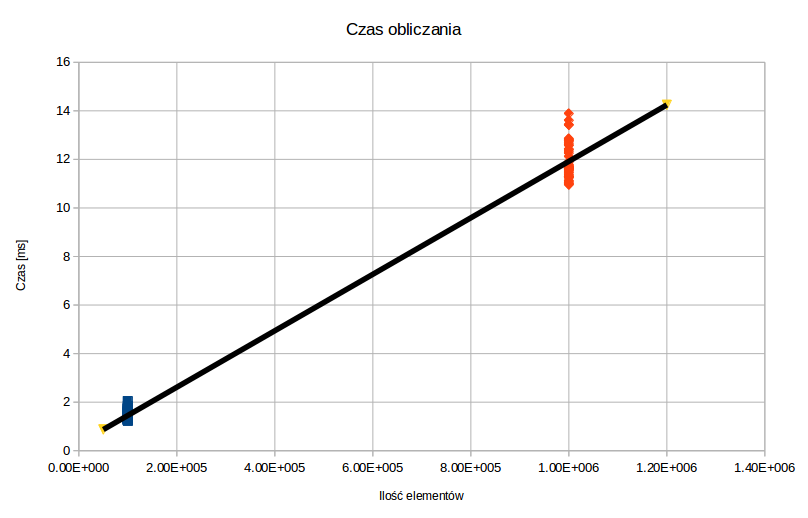
\includegraphics[scale=0.5]{../wykresy/stotysiecy-milion.png}
		\caption{Czas zapisu stu tysięcy oraz miliona intów oraz odpowiednia regresja liniowa}
	\end{center}
\end{figure}

\begin{figure}[hb]
	\begin{center}
		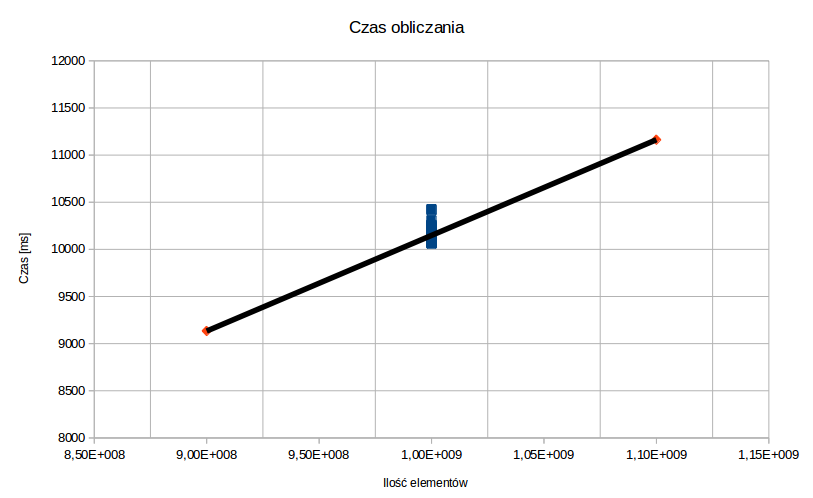
\includegraphics[scale=0.5]{../wykresy/miliard.png}
		\caption{Czas zapisu miliarda intów oraz odpowiednia regresja liniowa}
	\end{center}
\end{figure}


\section{Wnioski}
Zastosowanie nowego interfejsu znacznie zmniejszyło szanse na popełnienie błędu.
\end{document}